\section{Design Patterns}
When considering how to design a software solution it can be a good idea to consider using some design patterns. Without those, code easily becomes messy later on in the project. Patterns can help by providing conventions and best practices to use as guidelines. With defined patterns it can be ensured that everyone working on the project has similar understandings of the code. It is worth to note that like everything, patterns can be misused; It is important to choose those that will fit the project, rather than try to force harmful patterns on to it. 

Below is a description of patterns found usable in this project. Patterns are split into two, one with patterns applicable in the client application, another with patterns applicable on the server program.

\subsection{Patterns in the application}
%\textbf{Singleton} was an obvious pattern to use in the application for certain elements. Firstly, the application including all activities are singleton. This is enforced by Android. There is no reason why the user should run multiple instances of the game. A certain class called "Client" is however also important to keep singleton. This class is responsible for opening a connection to the server and handle communication. It should not be allowed for a user to send multiple requests to the server at once.

\textbf{Lazy Initialization} pattern is designed to save/delay use of resources by postponing initialization for as long as possible (Until right before it is needed).The Android application in this project does not perform many heavy operations, but it should always be remembered that the application is running on a phone with limitations in the form of battery life. As a mobile device, battery life is a valuable resource - a requirement for a mobile device is the ability to keep power for an extended period of time. As such, most initializations of objects has been pushed back to the point where they are required along with operations on data \cite{lazyInit}.

\textbf{Adapter} pattern is a simple idea, but can be used in many contexts. It stems from the problem of wanting two incompatible interfaces to work together. The pattern solution is to use adapters to facilitate a common ground for the two interfaces. In Android, adapters are used to construct lists, grids and more. The adapters help link lists of items together with a visualization, using a given layout to inflate and a set of items. It will then provide a view of each item, effectively providing a user-friendly way of using/viewing the data. The biggest problem with this pattern is that it requires writing code for delegating the requests to the adapted objects \cite{adappat}. For this project adapters have been used to create and display clickable lists.

\textbf{Facade} pattern describes the idea of hiding messy procedures by using a facade. The result is that whoever wants to use the procedures have access to simple, easy to use facades which acts as access points to the procedural steps \cite{facpat}. In this project it has been used mostly for abstracting away the server communication. As this is done by creating XML strings with relevant data, this would be tedious to do in every activity that needed server communication. The communication itself was also abstracted. Instead, this functionality has been written in separate classes and is accessed through simple method calls. An example can be seen in \ref{fig:facadepattern}. This displays what happens when a user tries to login. The username and password is converted to XML and sent to the server, which in turn provide a responde. All the details of how this happens are however hidden.

\begin{figure}[H]
\centering
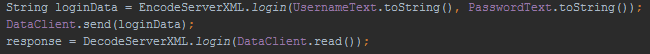
\includegraphics[width=\textwidth]{billeder/facadepattern.png}
\caption{Abstraction of server communication}
\label{fig:facadepattern}
\end{figure} 
% If you are about to write about thread pool, we are not using a thread pool. We just make a thread for each game.

% for pattern in project:
	%Describe each pattern we use:
	% - What is its purpose?
	% - Pros/cons?
	% - Alternatives?
	% - Flexibility (refactoring, adding new functionality, changing the pattern...)